\documentclass[]{article}
\usepackage{polski}
\usepackage[utf8]{inputenc}
\usepackage{amsmath}
\usepackage{multirow}
\usepackage{mathtools,leftidx}% http://ctan.org/pkg/{mathtools,leftidx}
\usepackage{graphicx}
\usepackage{float}

\usepackage[margin=0.7in]{geometry}


\title{Specyfikacja sterownika robota Velma}
\author{Jakub Postępski}
\date{7 stycznia 2019}

\begin{document}

\maketitle

Robot Velma (rys. \ref{fig:uc}) został skonstruowany w laboratorium robotyki. Posiada dwa ramiona sterowane impedancyjnie i może obracać tułowiem. Robot może działać w swojej przestrzeni konfiguracyjnej i operacyjnej.

\begin{figure}[H]
	\centering
	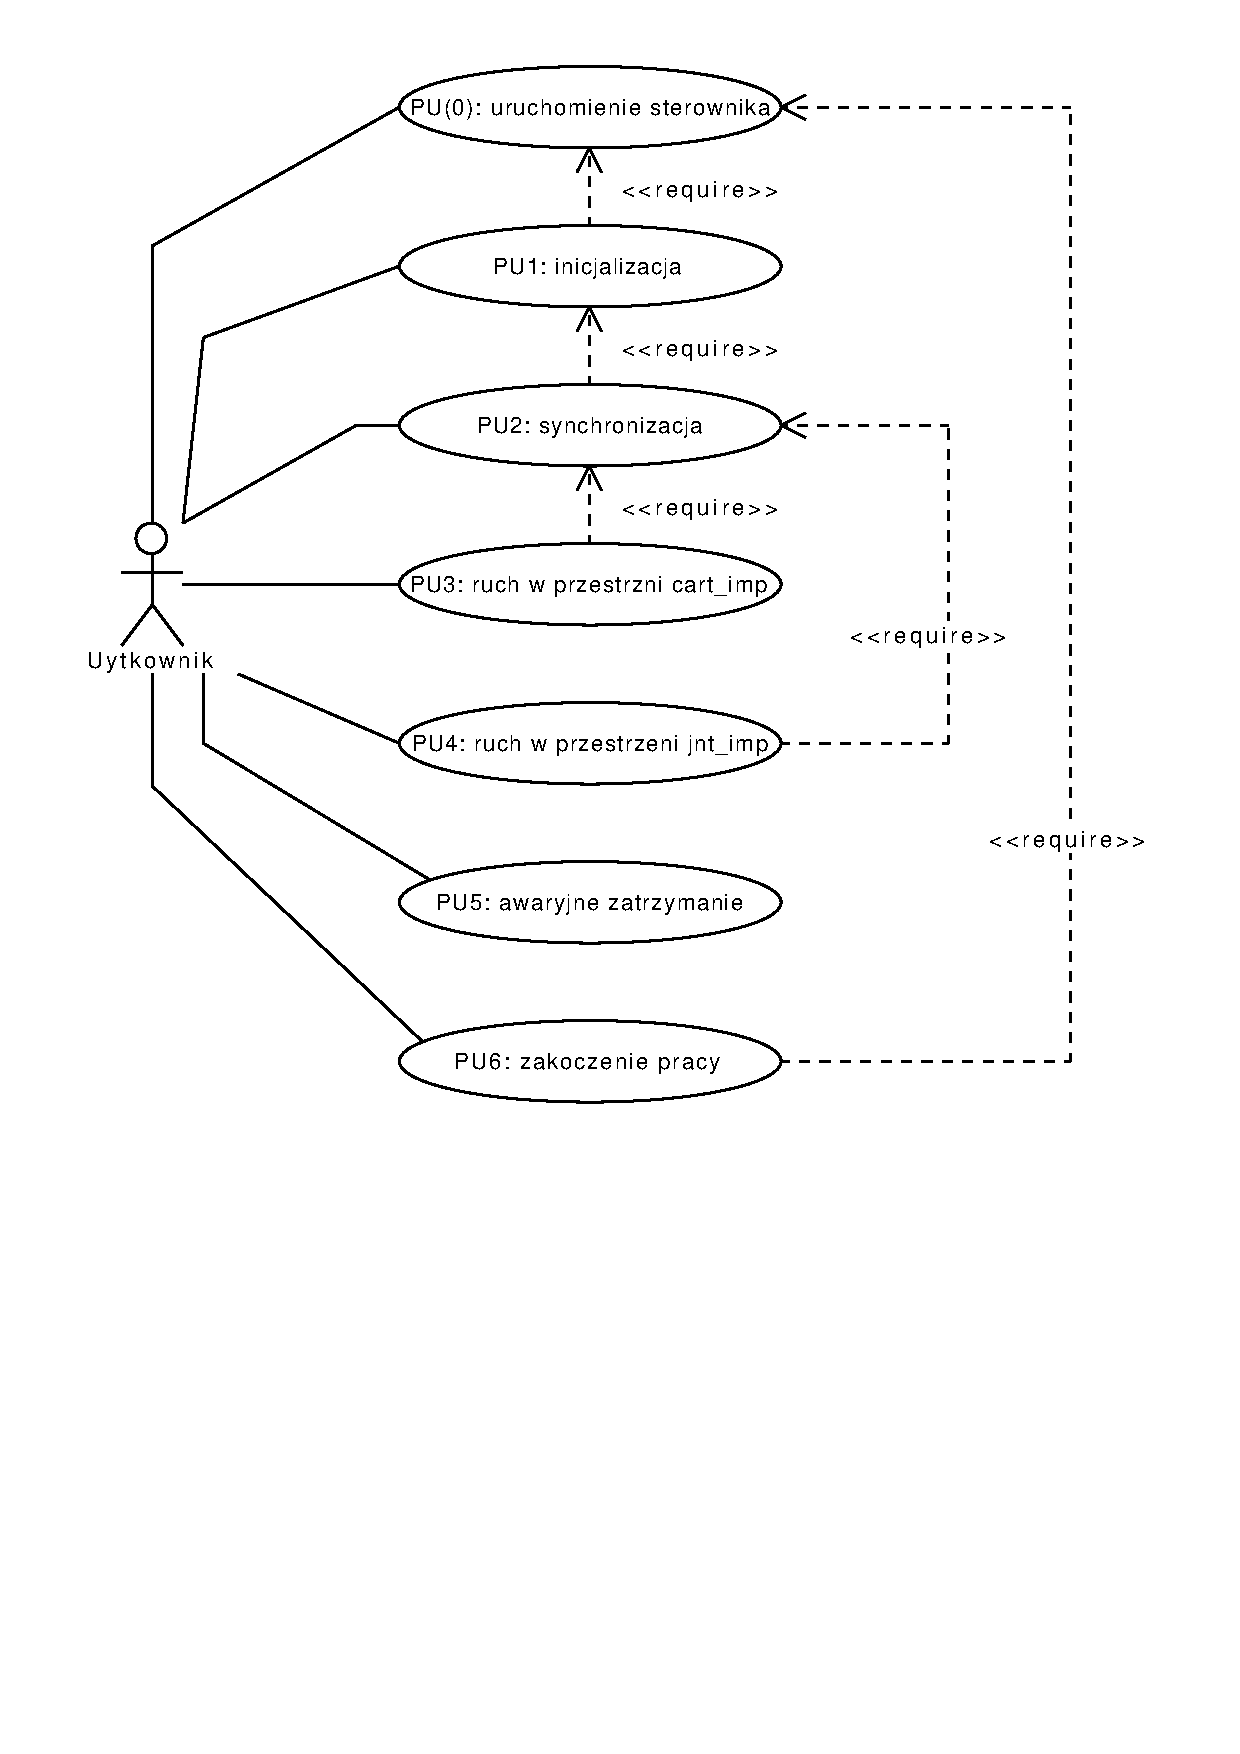
\includegraphics[width=0.7\linewidth]{velma}
	\caption{Przypadki użycia systemu}
	\label{fig:uc}
\end{figure}

\section{Struktura agentów systemu}
Sterownik robota został zdefiniowany jako dwa agenty (rys. \ref{fig:agents}). Agent \textbf{velma} steruje pracą robota i kontroluje jego urządzenia. Agent \textbf{velma\_ros\_interface} służy do wydawania poleceń dla robota i kontroli stanu.

W sprawozdaniu szczegółowo opisany jest tylko agent \textbf{velma}.

\begin{figure}[H]
	\centering
	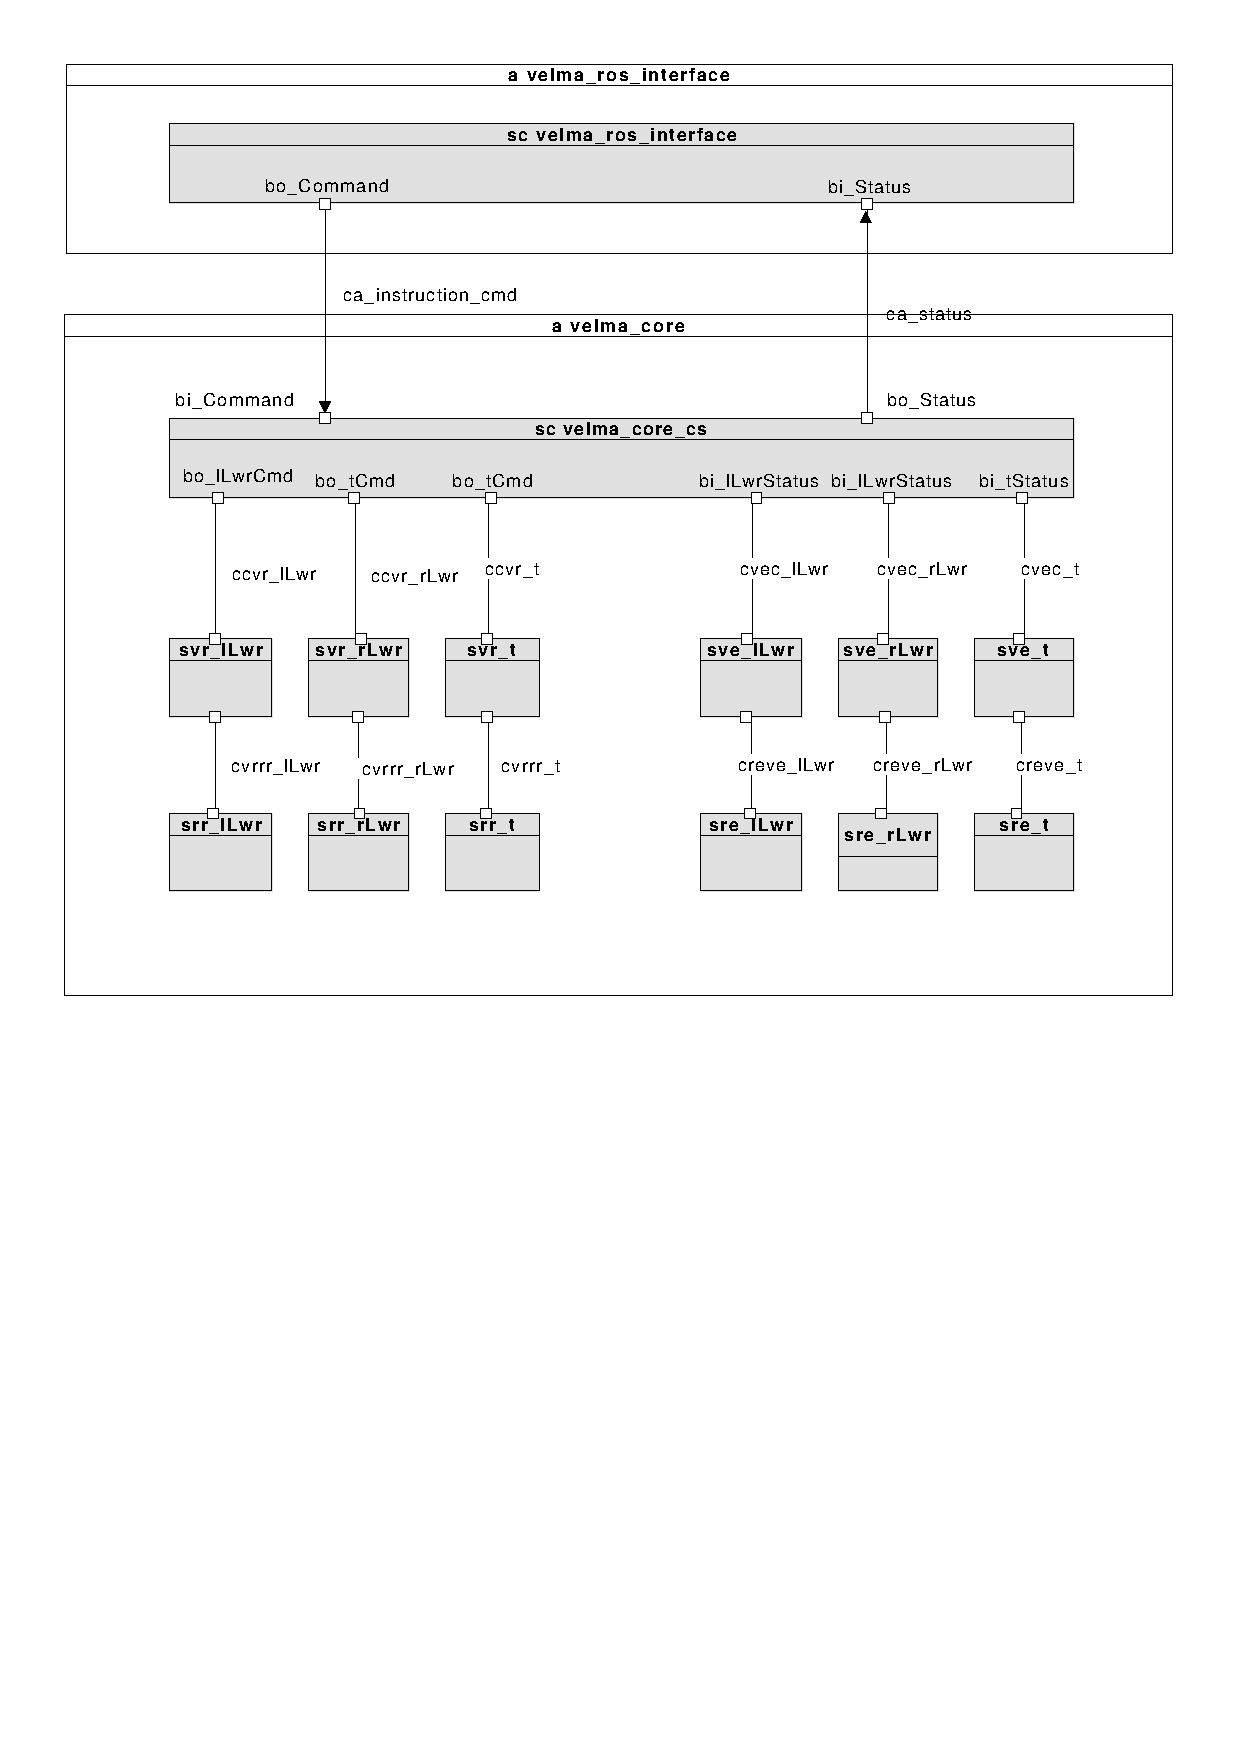
\includegraphics[width=0.8\linewidth]{main}
	\caption{Struktura agentów}
	\label{fig:agents}
\end{figure}

Poniżej przedstawiono zawartość kanałów informacyjnych robota.
\begin{table}[H]
	\begin{tabular}{||c|cc||}
		\hline\hline
		ca\_instruction\_cmd & Opis & Typ \\
		\hline\hline
		inst & instrukcje sterowania & struktura \\
		\hline\hline
		ca\_instruction\_st & Opis & Typ \\
		\hline\hline
		stat & status robota & struktura \\
		\hline
	\end{tabular}
	\label{tab:ca}
	\caption{Zawartość kanałów komunikacyjnych CA}
\end{table}


\begin{table}[H]
	\begin{tabular}{||c|cc||}
		\hline\hline
		ccve\_lLwrCmd & Opis & Typ \\
		\hline\hline

		lt & zadane momenty stawów lewego ramienia & float[7] \\
		\hline\hline
		ccve\_rLwrCmd & Opis & Typ \\
		\hline\hline

		rt & zadane momenty stawów prawego ramienia & float[7] \\
		\hline\hline
		ccve\_tCmd & Opis & Typ \\
		\hline\hline
		tq & zadany obrót tułowia & float \\
		th & polecenie zaczęcia synchronizacji obrotu tułowia & bool \\
		te & polecenie załączenia silnika tułowia & float \\
		\hline
	\end{tabular}
	\label{tab:ccve}
	\caption{Zawartość kanałów komunikacyjnych CCVE}
\end{table}

\begin{table}[H]
	\begin{tabular}{||c|cc||}
		\hline\hline
		cvec\_lLwrStatus & Opis & Typ \\
		\hline\hline
		lt & pozycja stawów lewego ramienia & float[7] \\
		ls & informacje diagnostyczne lewego ramienia & bool \\
		\hline\hline
		cvec\_rLwrStatus & Opis & Typ \\
		\hline\hline
		rs & informacje diagnostyczne prawego ramienia & bool \\
		rt & pozycja stawów prawego ramienia & float[7] \\
		\hline\hline
		cvec\_t & Opis & Typ \\
		\hline\hline
		tsh & synchronizacja stawu tułowia w toku & bool \\
		tse & silnik stawu tułowia aktywny & bool \\
		tsq & pozycja stawu tułowia & float \\
		\hline
	\end{tabular}
	\label{tab:cvec}
	\caption{Zawartość kanałów komunikacyjnych CVEC}
\end{table}


\section{Specyfikacja podystemu sterowania}

Podsystem sterowania robota (rys. \ref{fig:fsm}) ma za zadanie wykonywać zadania narzucone przez agenta \textbf{velma\_ros\_interface}. Jest odpowiedzialny za generację trajektorii oraz wyliczanie praw sterowania. Kontroluje podsystem wirtualnego efektora i zapobiega sytuacjom awaryjnym. Inicjalizuje włączanie i synchronizację silników.

Podstem działa w oparciu o maszynę stanów (rys. \ref{fig:fsm}). Stany są przełączane na podstawie predykatów (tab. \ref{tab:pred}).

	\begin{figure}[H]
		\centering
		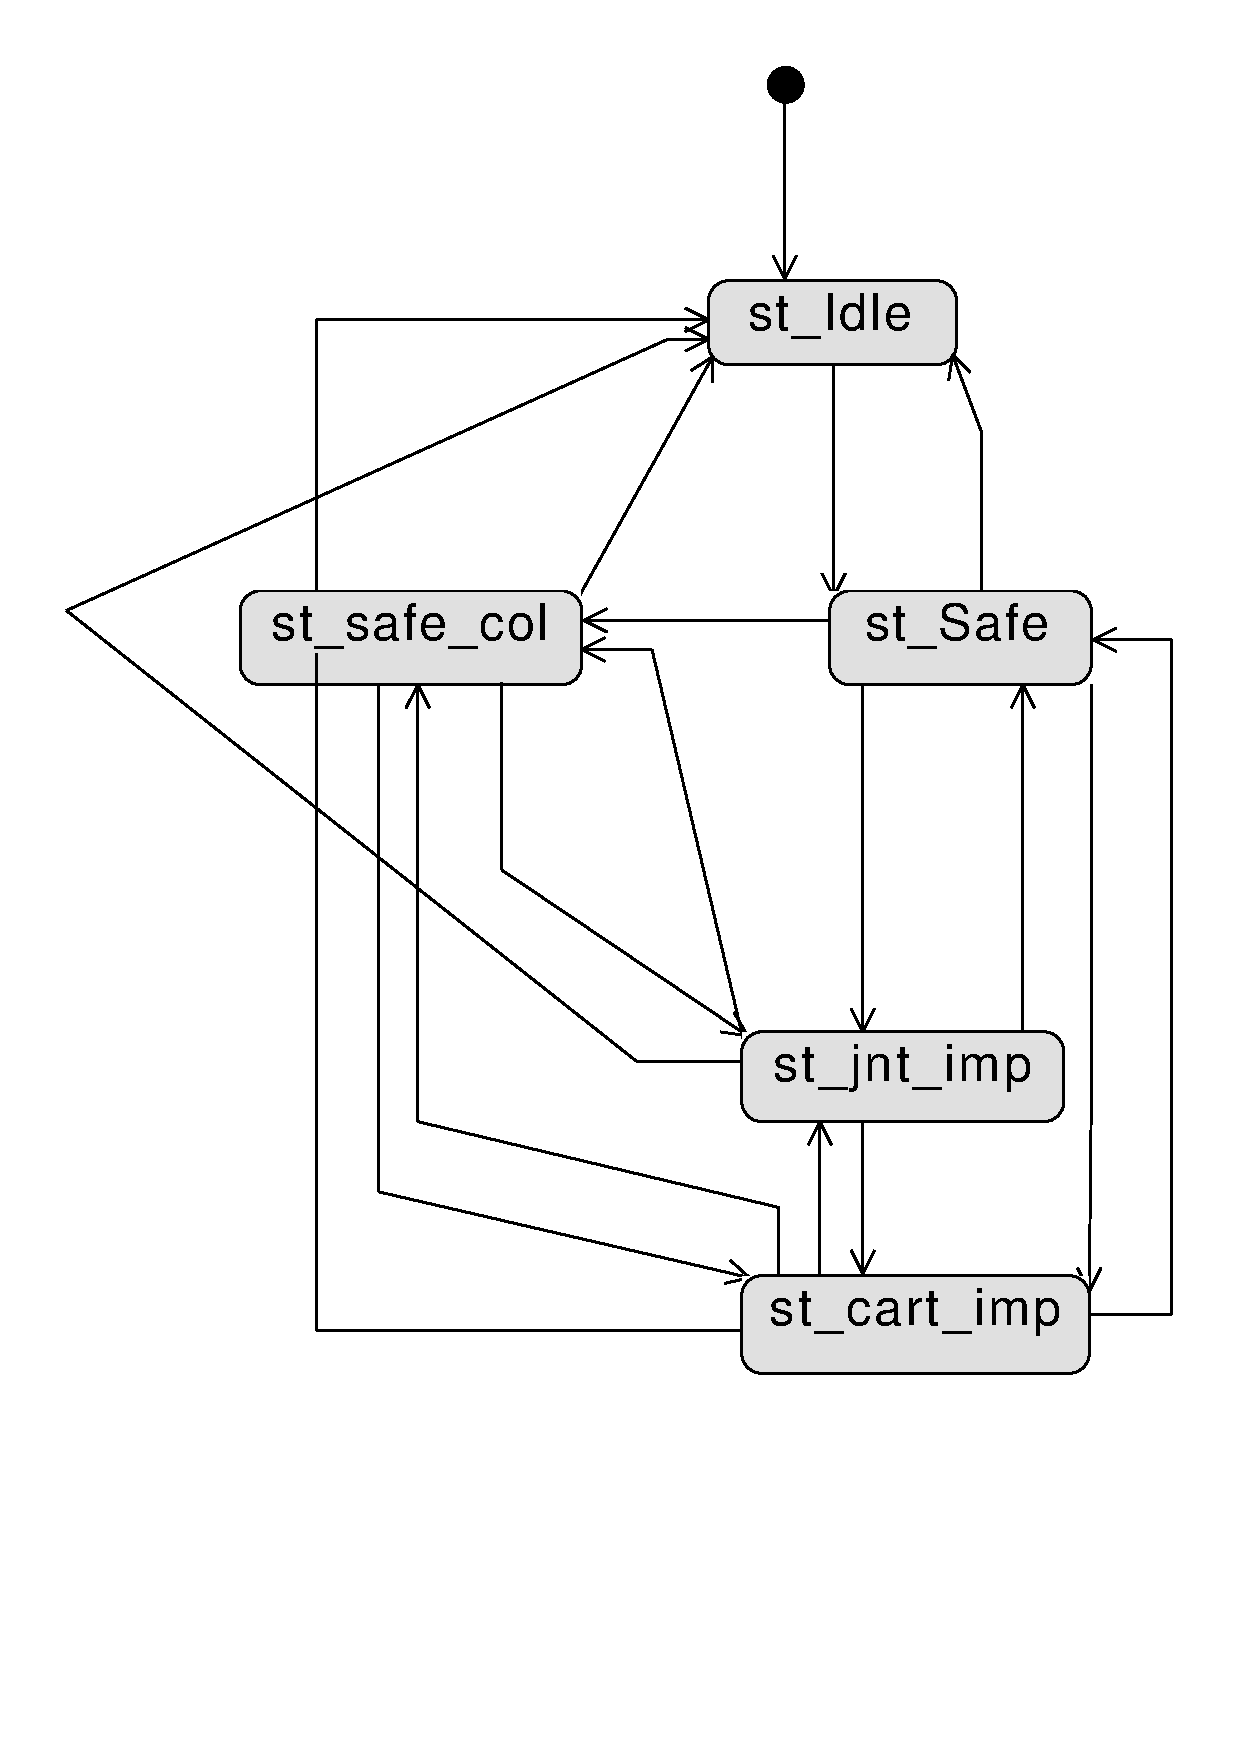
\includegraphics[width=0.4\linewidth]{fsm_cs}
		\caption{Automat skończony podsystemu sterowania}
		\label{fig:fsm}
	\end{figure}

	\begin{table}[H]
		\begin{tabular}{||c|c||}
		\hline
		Nazwa predykatu & Opis \\
		\hline \hline
		CURRENT\_BEHAVIOR\_OK & podsystem sterowania pracuje normalnie \\
		recvOneCmd & otrzymano dokładnie jedną wiadomość sterowania \\
		recvCartImpCmd & otrzymano wiadomość sterowania w trybie cart\_imp \\
		recvJntImpCmd & otrzymano wiadomość sterowania w trybie jnt\_imp \\
		recvSafeColCmd & otrzymano wiadomośc pracy w trybie safe\_col \\
		inSelfCollision & robot jest w stanie autokolizji \\
		IN\_ERROR & wykryto błąd systemu \\
		\hline
		\end{tabular}
		\label{tab:pred}
		\caption{Definicja predykatów}
	\end{table}


Do każdego stanu przyporządkowano zachowania (tab. \ref{tab:beh}). Zachowanie \textbf{idle} jest osiągane po włączeniu robota. Zachowanie \textbf{safeCol} pozwala poruszać się w trybie unikania kolizji. Zachowanie \textbf{cartImp} odpowiada sterowaniu w przestrzeni operacyjnej a zachowanie \textbf{jntImp} w przestrzeni konfiguracyjnej. Zachowanie \textbf{safe} jest osiągane przy wykryciu błędu systemu.

	\begin{table}[H]
		\begin{tabular}{||c|c||}
		\hline
		Stan & Zachowanie \\
		\hline \hline
		st\_idle & idle \\
		st\_safe & safe \\
		st\_cart\_imp & cart\_imp \\
		st\_jnt\_imp & jnt\_imp \\
		st\_safe\_cold & safe\_col \\
		\hline
		\end{tabular}
		\label{tab:beh}
		\caption{Przyporządkowanie zachowań do kolejnych stanów podsystemu sterowania}
	\end{table}

	\begin{table}[H]
		\begin{tabular}{||cc|c||}
		\hline
		Stan początkowy & Stan końcowy & Zachowanie \\
		\hline \hline
		st\_safe & st\_cart\_imp & $\neg{IN\_ERROR} \wedge recvCartImpCmd $ \\
		st\_safe & st\_jnt\_imp & $\neg{IN\_ERROR} \wedge recvJntImpCmd $ \\
		st\_safe & st\_safe\_col & $\neg{IN\_ERROR} \wedge recvSafeColCmd $ \\
		st\_safe\_col & st\_cart\_imp & $\neg{IN\_ERROR} \wedge recvCartImpCmd $ \\
		st\_safe\_col & st\_jnt\_imp & $\neg{IN\_ERROR} \wedge recvJntImpCmd $ \\
		st\_cart\_imp & st\_safe & $\neg{IN\_ERROR} \wedge \neg{recvOneCmd} $ \\
		st\_cart\_imp & st\_jnt\_imp & $\neg{IN\_ERROR} \wedge \neg{recvOneCmd} \wedge recvJntImpCmd $ \\
		st\_cart\_imp & st\_safe\_col & $\neg{IN\_ERROR} \wedge \neg{recvOneCmd} \wedge recvSafeColCmd $ \\
		st\_jnt\_imp & st\_safe & $\neg{IN\_ERROR} \wedge \neg{recvOneCmd} $ \\
		st\_jnt\_imp & st\_cart\_imp & $\neg{IN\_ERROR} \wedge \neg{recvOneCmd} \wedge recvCartImpCmd $ \\
		st\_jnt\_imp & st\_safe\_col & $\neg{IN\_ERROR} \wedge \neg{recvOneCmd} \wedge recvSafeColCmd $ \\
		dowolny & idle & $IN\_ERROR$\\
		\hline
		\end{tabular}
		\caption{Warunki przejść pomiędzy stanami podsytemu sterowania}
	\end{table}
\newpage
Przykładowa funkcja przejścia \textbf{jntMove} (tab. \ref{tab:fp}, rys. \ref{fig:jnt}) jest odpowiedzialna za wykonanie ruchu w przestrzeni konfiguracyjnej.

\begin{figure}[H]
	\centering
	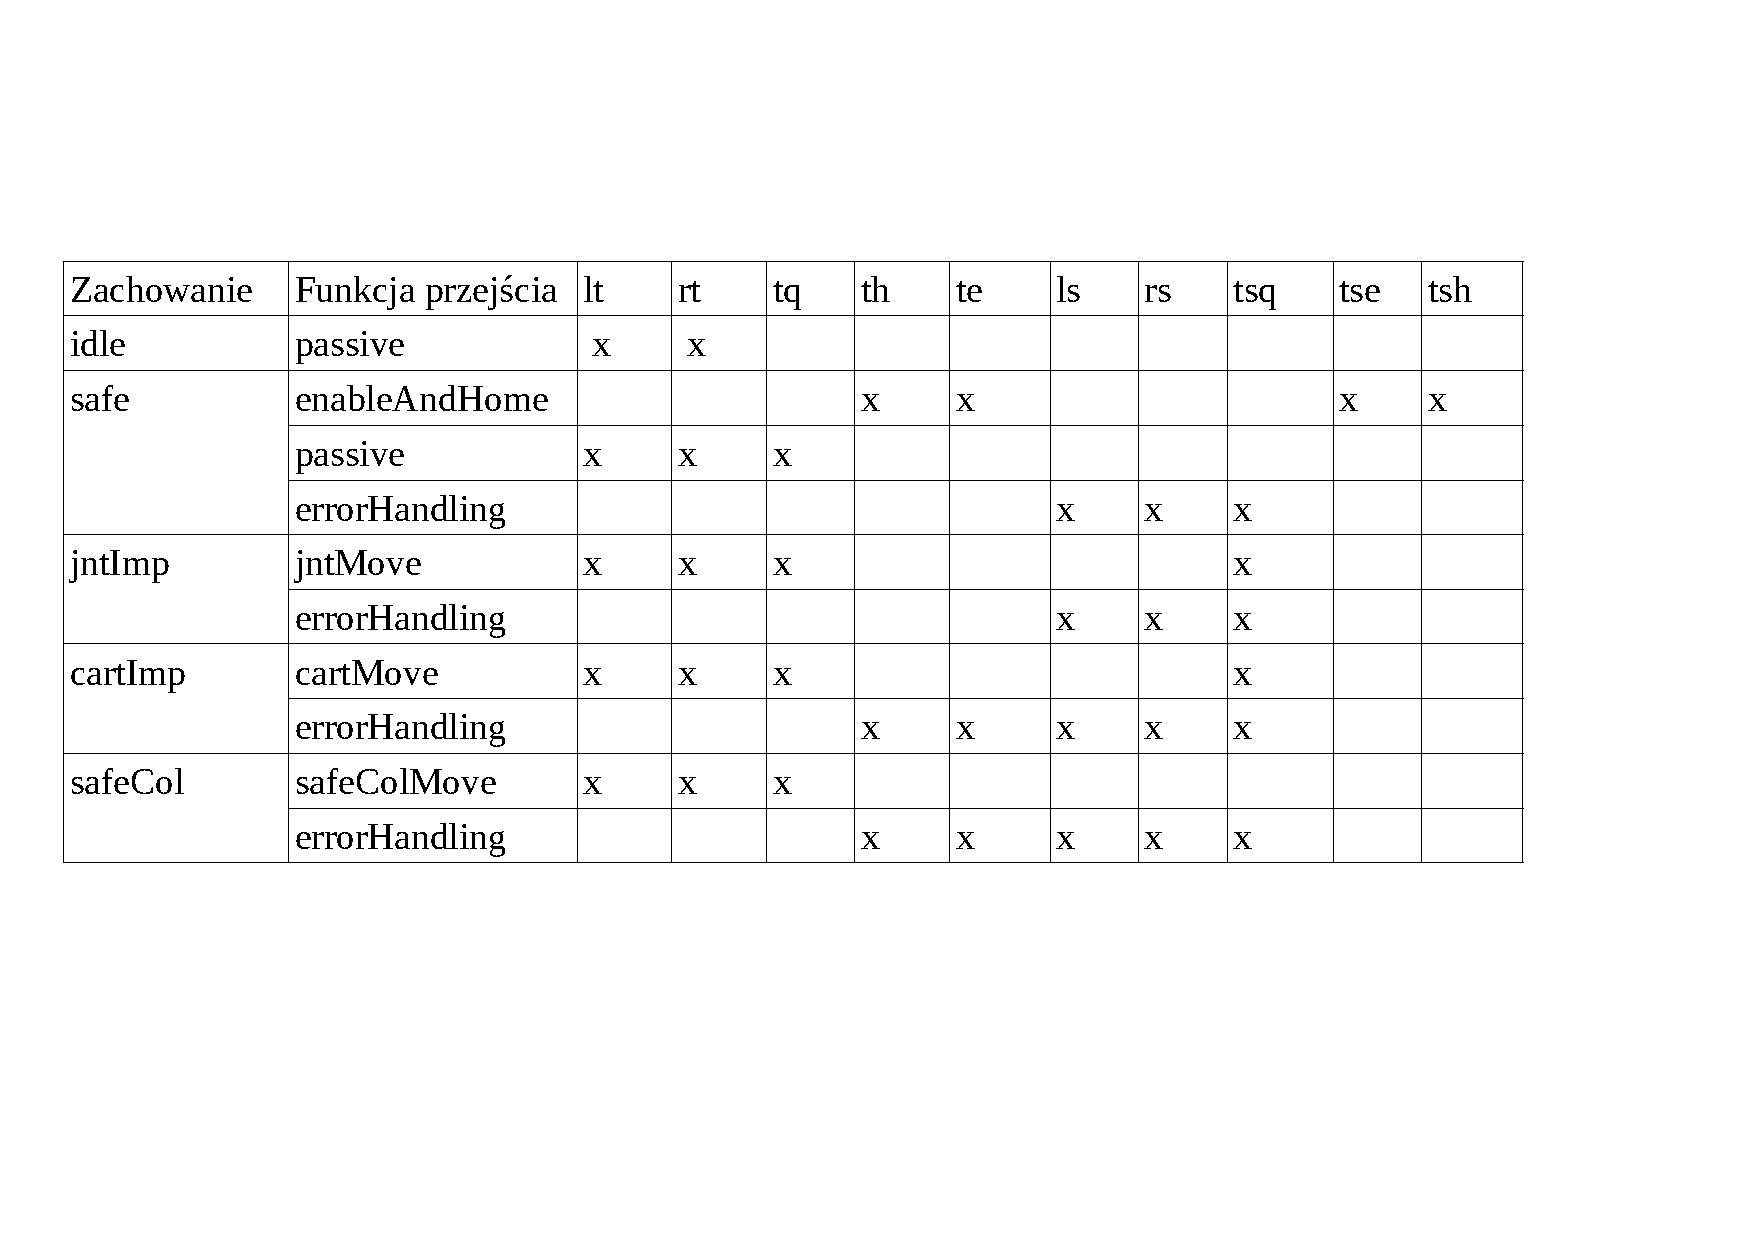
\includegraphics[width=0.9\linewidth]{przejscia}
	\caption{Kompozycja funkcji przejść}
	\label{tab:fp}
\end{figure}

\begin{figure}[H]
	\centering
	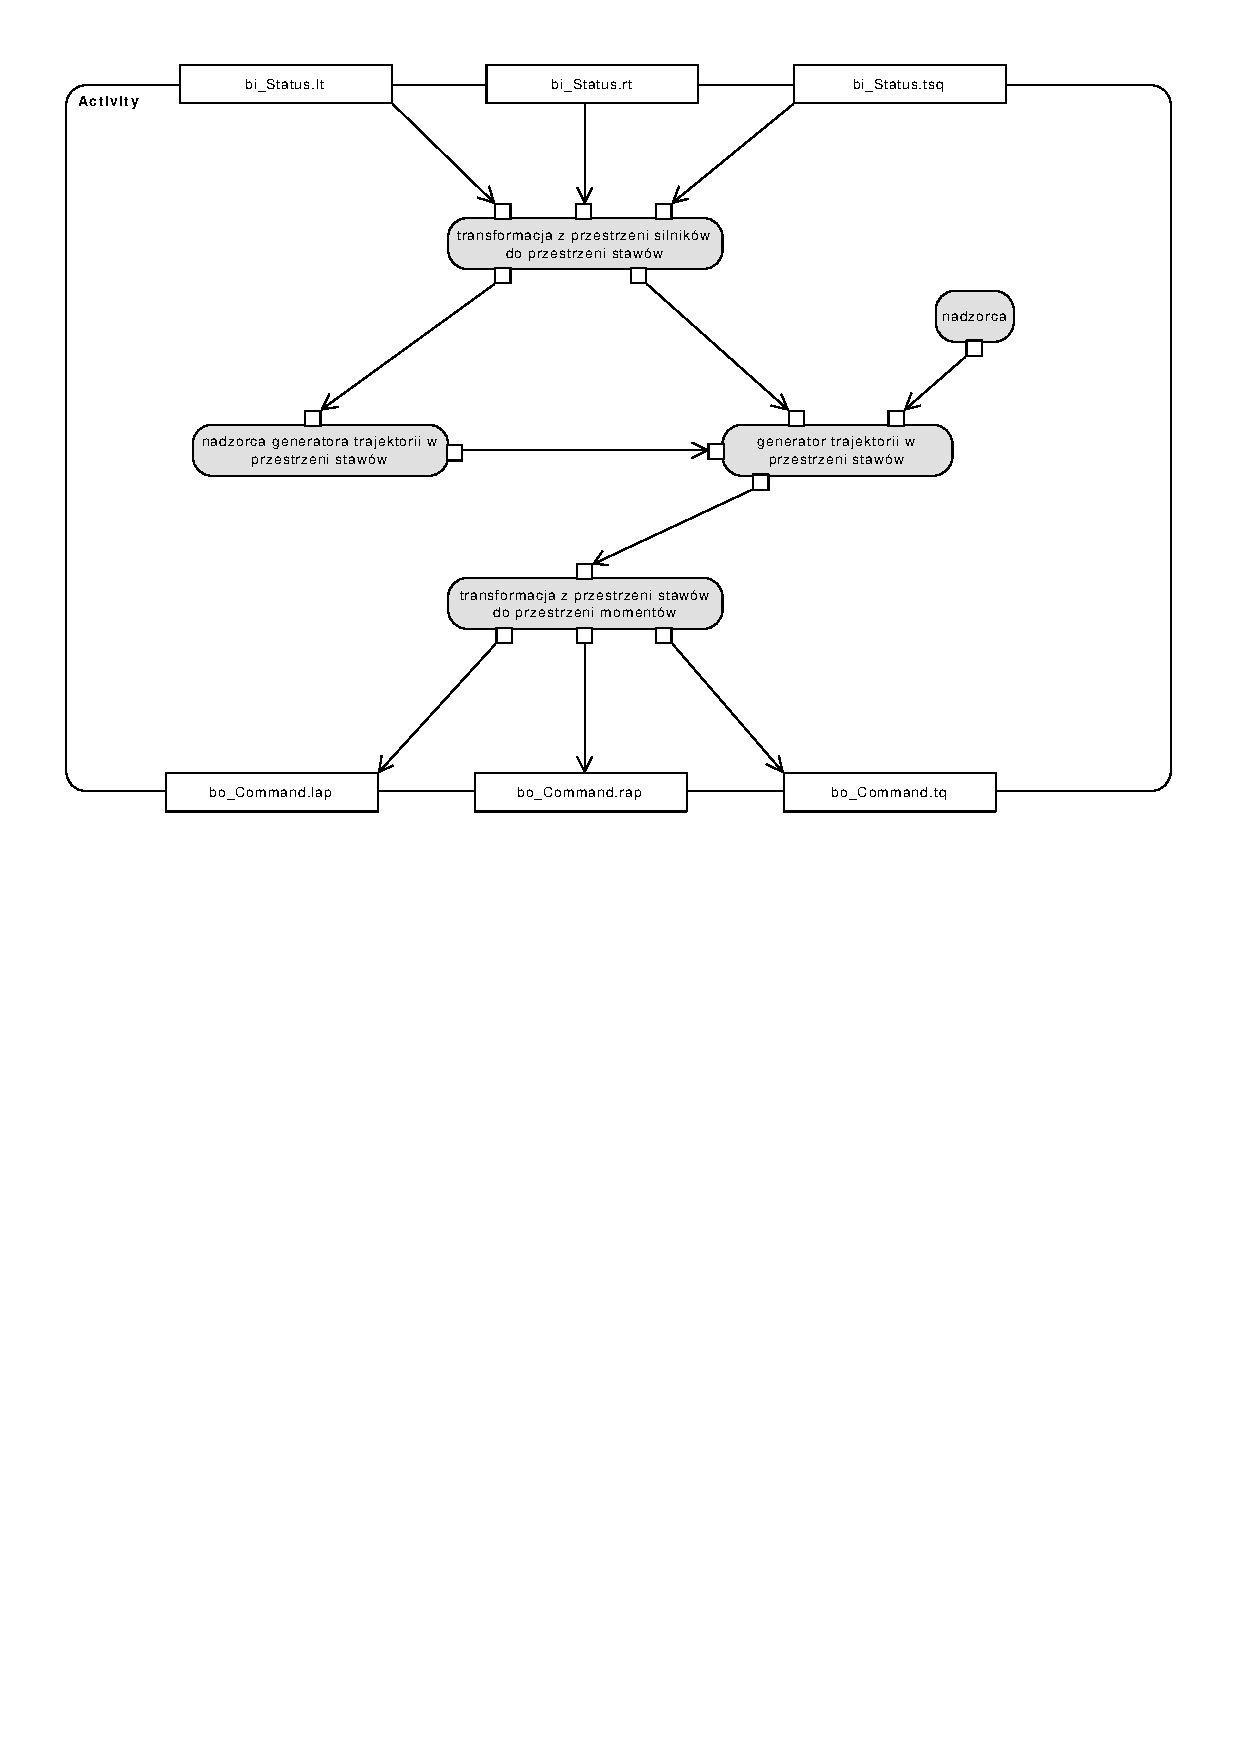
\includegraphics[width=0.9\linewidth]{jntMove}
	\caption{$Fp$ jntMove}
	\label{fig:jnt}
\end{figure}

\end{document}